% This is "sig-alternate.tex" V2.0 May 2012
% This file should be compiled with V2.5 of "sig-alternate.cls" May 2012
%
% This example file demonstrates the use of the 'sig-alternate.cls'
% V2.5 LaTeX2e document class file. It is for those submitting
% articles to ACM Conference Proceedings WHO DO NOT WISH TO
% STRICTLY ADHERE TO THE SIGS (PUBS-BOARD-ENDORSED) STYLE.
% The 'sig-alternate.cls' file will produce a similar-looking,
% albeit, 'tighter' paper resulting in, invariably, fewer pages.
%
% ----------------------------------------------------------------------------------------------------------------
% This .tex file (and associated .cls V2.5) produces:
%       1) The Permission Statement
%       2) The Conference (location) Info information
%       3) The Copyright Line with ACM data
%       4) NO page numbers
%
% as against the acm_proc_article-sp.cls file which
% DOES NOT produce 1) thru' 3) above.
%
% Using 'sig-alternate.cls' you have control, however, from within
% the source .tex file, over both the CopyrightYear
% (defaulted to 200X) and the ACM Copyright Data
% (defaulted to X-XXXXX-XX-X/XX/XX).
% e.g.
% \CopyrightYear{2007} will cause 2007 to appear in the copyright line.
% \crdata{0-12345-67-8/90/12} will cause 0-12345-67-8/90/12 to appear in the copyright line.
%
% ---------------------------------------------------------------------------------------------------------------
% This .tex source is an example which *does* use
% the .bib file (from which the .bbl file % is produced).
% REMEMBER HOWEVER: After having produced the .bbl file,
% and prior to final submission, you *NEED* to 'insert'
% your .bbl file into your source .tex file so as to provide
% ONE 'self-contained' source file.
%
% ================= IF YOU HAVE QUESTIONS =======================
% Questions regarding the SIGS styles, SIGS policies and
% procedures, Conferences etc. should be sent to
% Adrienne Griscti (griscti@acm.org)
%
% Technical questions _only_ to
% Gerald Murray (murray@hq.acm.org)
% ===============================================================
%
% For tracking purposes - this is V2.0 - May 2012

\documentclass{sig-alternate}

\usepackage{etoolbox}		% for \newbool, \setbool, etc.
\usepackage{color}		% colors, obviously
\usepackage{xspace}		% handy for macros that need a space after them sometimes. 
\usepackage{microtype}		% sets text smaller
\usepackage{graphicx}		%
\usepackage{subcaption}		%
\usepackage{url}		%

\newbool{inccomment}
% set to false to exclude comments from the output
\setbool{inccomment}{true}
\newcommand{\fixme}[1]{\ifbool{inccomment}{{\color{blue}FIXME: #1}}{}}
\newcommand{\gulp}[1]{}{}

% Make enumerations that don't have as much inter-line spacing.
% Thanks to jdh8d.
\newenvironment{packed_enumerate}{
\begin{enumerate}
	\setlength{\itemsep}{0.25em}
	\setlength{\parskip}{0pt}
	\setlength{\parsep}{0em}
}{\end{enumerate}}

\newenvironment{packed_itemize}{
\begin{itemize}
	\setlength{\itemsep}{0.25em}
	\setlength{\parskip}{0pt}
	\setlength{\parsep}{0em}
}{\end{itemize}}

% useful if we want to change the name sometime.

\pagenumbering{arabic}  % Arabic page numbers GM July 2000


\begin{document}
%
% --- Author Metadata here ---
%\conferenceinfo{WOODSTOCK}{'97 El Paso, Texas USA}
%\CopyrightYear{2007} % Allows default copyright year (20XX) to be over-ridden - IF NEED BE.
%\crdata{0-12345-67-8/90/01}  % Allows default copyright data (0-89791-88-6/97/05) to be over-ridden - IF NEED BE.
% --- End of Author Metadata ---

\title{UpvoteetovpU: Looping GIFs}
%\subtitle{[Extended Abstract]
%\titlenote{A full version of this paper is available as
%\textit{Author's Guide to Preparing ACM SIG Proceedings Using
%\LaTeX$2_\epsilon$\ and BibTeX} at
%\texttt{www.acm.org/eaddress.htm}}}
%
% You need the command \numberofauthors to handle the 'placement
% and alignment' of the authors beneath the title.
%
% For aesthetic reasons, we recommend 'three authors at a time'
% i.e. three 'name/affiliation blocks' be placed beneath the title.
%
% NOTE: You are NOT restricted in how many 'rows' of
% "name/affiliations" may appear. We just ask that you restrict
% the number of 'columns' to three.
%
% Because of the available 'opening page real-estate'
% we ask you to refrain from putting more than six authors
% (two rows with three columns) beneath the article title.
% More than six makes the first-page appear very cluttered indeed.
%
% Use the \alignauthor commands to handle the names
% and affiliations for an 'aesthetic maximum' of six authors.
% Add names, affiliations, addresses for
% the seventh etc. author(s) as the argument for the
% \additionalauthors command.
% These 'additional authors' will be output/set for you
% without further effort on your part as the last section in
% the body of your article BEFORE References or any Appendices.

\numberofauthors{2} %  in this sample file, there are a *total*
% of EIGHT authors. SIX appear on the 'first-page' (for formatting
% reasons) and the remaining two appear in the \additionalauthors section.
%
\author{
% You can go ahead and credit any number of authors here,
% e.g. one 'row of three' or two rows (consisting of one row of three
% and a second row of one, two or three).
%
% The command \alignauthor (no curly braces needed) should
% precede each author name, affiliation/snail-mail address and
% e-mail address. Additionally, tag each line of
% affiliation/address with \affaddr, and tag the
% e-mail address with \email.
%
% 1st. author
\alignauthor
Will~Hawkins and Jamie~Floyd\\
	\affaddr{Computer Science Department, Univ. of Virginia}\\
%	\affaddr{University of Virginia}\\
	\email{\{whh8b,bef2cj\}@virginia.edu}
}
\date{28 April 2014}

\maketitle
\section{Abstract}
\label{sec:Abstract}
After the invention of the GIF file format in 1987 and their popularization in social media, the task of selecting interesting segments from videos has become important. Similarly, tools that assist users in accomplishing this task have become highly valued. While there are many conceptions of what makes an \textit{interesting}, the looping GIF has become incredibly popular. There exist several tools to help users create GIFs from videos, but the task of finding the perfect start and end frame to create a seamless loop must be done by hand. While this approach allows creativity, it is difficult and offers no guarantees that the best frames will be selected. Driven by this need for a better method of selecting proper frame pairs for perfectly looping GIF, we have created UpvoteetovpU, a tool that automatically extracts GIFs from an input video. 

In this paper, we describe UpvoteetovpU's distance metric that calculates differences between frames of a video, method for extracting perfect loops from a video based on that metric, method of creating and applying a mask to frames of a video for interesting effects and optimizations on those methods.

%A category including the fourth, optional field follows...
\gulp{
\category{D.3.4}{Programming Languages}{Processors}[Code Generation, Compilers, Optimization]

\terms{Algorithms, Measurement, Performance, Design, Experimentation}

\keywords{Static rewriting, binary rewriting, static analysis}
}
\section{Introduction}
\label{sec:Introduction}
After the invention of the GIF file format in 1987 and their popularization in social media, the task of selecting interesting segments from videos has become important. Similarly, tools that assist users in accomplishing this task have become highly valued. While there are many conceptions of what makes an \textit{interesting} video segment, we focus on a definition that is particularly relevant to the GIF format: because GIFs loop back from their last frame to their first frame in an endless cycle, detecting perfect loops in videos creates a GIF depicting a scene that goes on forever without showing the \textit{seam} -- the transition from the last frame back to the first frame. This type of GIF has become incredibly popular, gaining its own subreddit (www.reddit.com/r/perfectloops/) as well as many other mediums. There exist several tools to help users create GIFs from videos, but the task of finding the perfect start and end frame to create a seamless loop must be done by hand. While this approach allows creativity, it is difficult and offers no guarantees that the best frames will be selected. Driven by this need for a better method of selecting proper frame pairs for perfectly looping GIF, we have created a tool that automatically extracts GIFs from an input video. It makes a selection of start and end frames by comparing how similar they are in a mathematical way. 

Another technique that is being applied to GIF creation is the alteration of the original images of a video. This could include color segmentation, adding text, and many other effects. In addition to automatic loop detection, our work makes use of a masking technique - highlighting the interesting parts of each frame - to apply one such effect. 

In this paper, our contributions and key implementation ideas are as follows:
\begin{itemize}
  \item A distance metric between frames of a video
  \item A method for extracting perfect loops from a video based on that metric
  \item A method of creating and applying a mask to frames of a video for interesting effect generation
  \item Methods for optimizing this process for time
\end{itemize}

\section{Prior Work}
\label{sec:PriorWork}
Several tools have been developed to aid a user in creating a GIF from a video. Popular options include makeagif.com, memecenter.com, and Jiffy (a Google Chrome extension to Youtube).
Each of these tools has its benefits and drawbacks. However, all of them require manual selection of start and end frames of the video segment that will be used to create a GIF. 

There has been some work in the field of automated loop detection: Loop Findr, a project of Collin Burger at Carnegie Mellon, is designed to scan movies and extract any perfectly looping segments within them. However, this tool has no methods to alter the frames of a video. While Loop Findr is able to tackle very large videos, that is the extent of its functionality. 

\section{Design and Implementation}
\label{sec:DesignImplementation}
\subsection{Algorithmic Design}
\label{sec:AlgorithmicDesign}
\subsubsection{Definitions}
\label{sec:Definitions}
A \textit{frame} is a two-dimensional array of pixels and a \textit{video} is a sequence of frames. Depending on the type of video, the frames may be grayscale (in which case each pixel contains a single scalar value) or color (in which case pixels contain multiple values that represent color channels). A video can be indexed with a particular index $i$ to retrieve the $i^{th}$ frame as long as $i$ is less than $l$, the total number of frames in the video. 
An \textit{approximate frame} $f'$ is a frame derived from another frame $f$. $f'$'s pixel values are related to $f$'s pixel values according to some function. Depending on the function, $f'$ may contain less or as much information as $f$. As the name implies, however, it is often the case that $f’$ contains less information than f. 
Let $D$ be a function that takes an input video $v$ and two indexes $x$ and $y$ and returns a scalar result. The result of $D(v, x,y)$ is the distance between the frames $x$ and $y$ in the video $v$. There are many different possible ways to define $D$ and calculate the distance. Our definition is based on Euclidean distance and outlined below in detail.
We define a \textit{video sequence} as a pair of indices $(x,y)$ where $x$ is greater than $y$ and $x$ and $y$ are less than $l$. A video sequence $(x,y)$ for video $v$ is \textit{well-looping} if $D(v,x,y) < T$ where $T$ is a threshold value. A \textit{video loop} is a well-looping video sequence $(x,y)$ for video $v$.
\subsubsection{Distance}
\label{sec:Distance}
The distance metric used in our approach is based on the Euclidean distance. It is as follows:
$$d(F_1,  F_2) = \sqrt{\sum_{i=1}^N (F_1[i] -  F_2[i])^2}.$$
Note that the above metric is for intensity images. The core idea still applies to full color images; the internal subtraction is just done in each color channel. 

This distance metric is simple enough to implement: the full color version is shown in pseudocode below.
\begin{verbatim}
def d(im1, im2):
  i1_s = im1.shape
  i2_s = im2.shape
  distance = 0
   for x in range(i1_s[0]):
    for y in range(i1_s[1]):
     for z in range(i1_s[2]):
      if im1[x][y][z] == im2[x][y][z]:
       continue
      distance += abs(im1[x][y][z] 
       - im1[x][y][z])**2
     return (distance /
       (i1_s[0] * i1_s[1] * i1_s[2]))**(1/2)
\end{verbatim}
Despite its simplicity, most of our distance calculations do not follow this implementation. We rewrite it in a mathematically equivalent way, according to the law of consines. The above equation can be reformed into the following:
																																														$$d(F_1,  F_2) = \sqrt{ \|F_1\|_2^2 + \| F_2\|_2^2 - 2 (F_1 \cdot  F_2) }$$
																																														where the notations are used
																																														$$\|F\|_2^2 = \sum_{i=1}^N F[i]^2,  \,\,\,\,\,\,\, F_1 \cdot F_2 =  \sum_{i=1}^N F_1[i]F_2[i]$$
																																														This form of the distance equation performs the same as the original, but has an added benefit: because $\|F\|_2^2$ depends only on a single frame (and not a pair of frames), it can be precomputed. This leaves the actual distance formula with fewer calculations. The original had approximately $3N$ calculations: $N$ subtractions, $N$ multiplications, and $N-1$ additions. The new distance formula, with the norms precomputed only requires $2N$ calculations, resulting in an overall speedup. 
\subsubsection{Masks}
\label{sec:Masks}
Masks can be used to filter or replace pixel values in the frames of a video \cite{Piccardi2004}. For example, a mask can filter out all the blue in the frames of a video or replace all pixels outside a particular region with pixels from an external image. A mask might also indicate the region of frames where interesting motion exists throughout a video. 
In the scope of this project, we define the mask as a single two-dimensional array with the same height and width as the frames of the video. The mask may also have associated data (used to make filtering decisions, define replace values, etc). 
Masks can serve two purposes in building video loops: functional and aesthetic. Functionally, masks may help the loop detection algorithm stabilize a shaky input video. A mask could define the moving parts of the video and build approximate frames from that subregion. A user could define a mask as a hint to the loop detection algorithm. We did not implement functional masks in the current version of the system.
Aesthetic masks affect the look of the video produced by the system. For example, they could be used to define the regions of the frames that should be replaced with a solid color or cropped out entirely. We implemented two different aesthetic masks: colorize and background. The colorize mask is used to define a region of pixels of a frame that should retain their original color values -- pixels outside the region will be converted to grayscale. The background mask defines a region of pixels of a frame that should be replaced with pixel values from some external image. 
In the system, masks can be defined according to the median and mean values of a pixel across a video. Masks are applied to frames depending on the difference between the actual value of a pixel and the median (mean) value of that pixel throughout the video. As mentioned above, each mask defines a way to alter the pixel value when the difference exceeds the threshold. 
\subsubsection{Pipeline}
\label{sec:Pipeline}
\begin{figure*}
\centering
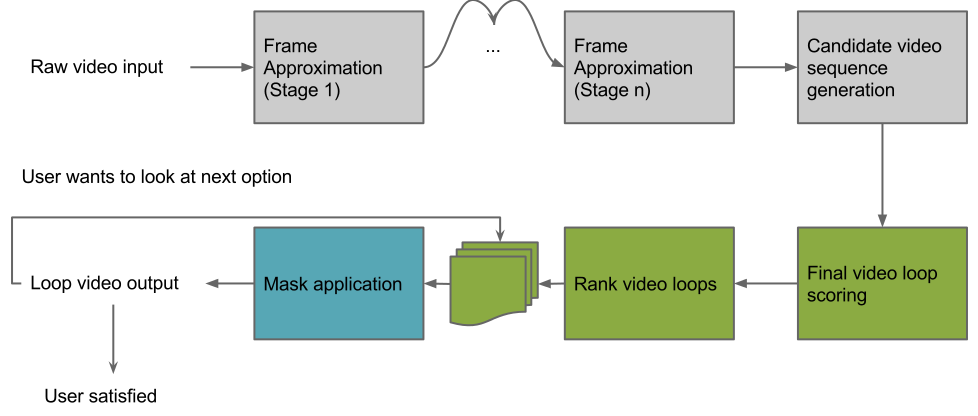
\includegraphics[width=1.0\textwidth]{loop-pipeline.png}
\caption{Overall workflow of UpvoteetovpU}
\label{fig:Pipeline}
\end{figure*}
The final pipeline for our approach is as follows: first, user parameters are read and their effects are implemented. The possible parameters are shown by example:
\begin{itemize}
\item \textbf{-o all} : Performs optimization based on edges and downsampling
\item \textbf{-l 1s -m 7s} : Restricts the output length to be between 1 second and 7 seconds. If parameters do not include the `s', they will be treated as frame counts
\item \textbf{-s 100 -e 250} : Restricts the algorithm's search space to starting at the $100^{th}$ line and ending at the $250^{th}$ line
\item \textbf{-t 20} : sets the threshold for determining which frame pairs are testing in full colorspace (is meaningless if no optimization is used)
\item \textbf{-i} : Runs in interactive mode, allowing user to see more than just the single best output
\end{itemize}

With these parameters set, the next step in the pipeline is to create the relevant Video objects. If the user has opted to compute any approximations for an optimization (such as edge frames or scaled frames), those are computed. Then, the approximation is run through a function that computes the distance between all relevant pairs of frames. It returns a list of frame pairs and distances that is then sorted for distance. All of the candidate pairs from the approximations that have a distance below the set threshold are run through the full color distance function. Those results are also sorted for distance. Then, the best frame pair for creating a perfect loop is the first item in the sorted list. In regular mode, a GIF is created with those endpoints. In interactive mode, the user can opt to get the next-best result if the current one is not desirable.

\subsection{Implementation Design}
\label{sec:ImplementationDesign}
The system is implemented in Python and uses a set of external libraries. The system relies on NumPy \cite{NumPy}, OpenCV \cite{OpenCV}, and skimage \cite{skimage}. In the following sections, we describe, at a high level, the implementation of the system.
\subsubsection{Video}
\label{sec:Video}
A \textit{video} is implemented as a \texttt{Video} object. Each video object has certain properties (like the name of the source video file if it was created from a file stored on disk, the total number of frames, etc) and certain methods. 
The frames of the video are stored as an array within the video object. Each frame of a video is accessible through the \texttt{[i]} operator where $i$ is the frame index. The result of the \texttt{[i]} operation is a frame -- a two-dimensional array whose individual objects are formatted according to the type of video. The \texttt{[i:j]} operator, where $i$ and $j$ are frame indexes and $j>i$, creates a new \texttt{Video} whose contents are the frames from $i$ to $j$, inclusive. 
A \texttt{Video} knows how to turn itself into an animated GIF and store the output into a file. A video also knows how to iterate through itself in an idiomatic Python way. 
There are three subclasses of \texttt{Video} (\texttt{GrayVideo}, \texttt{EdgeVideo} and \texttt{ScaleVideo}) that can be instantiated from existing \texttt{Video} objects or from videos stored in files on disk. When a \texttt{GrayVideo} is instantiated, the frames are immediately converted to grayscale. When an \texttt{EdgeVideo} is instantiated, its frames are immediately run through a Canny edge detector. When a \texttt{ScaleVideo} is instantiated, its frames are immediately scaled to a new size. By instantiating one of these subclasses from an existing \texttt{Video} object, a video of approximate frames is immediately available. It is possible to ``chain'' instantiations so that the approximations can be applied one-after-another. 
\subsubsection{Mask}
\label{sec:Mask}
A \textit{mask} is implemented as a \texttt{Mask} object. Each mask object has certain properties (like a threshold value) and certain methods and requires at least a \texttt{Video} object \textit{v} as a parameter for construction. The frames of \textit{v} determine the values of the mask depending on the type of mask. These mask values are stored as a two-dimensional array within the object. A mask value at pixel $(i,j)$ is accessible by indexing a mask object using \texttt{[i][j]}. 
A \texttt{Mask} implements a \texttt{decide} function. \texttt{decide} takes three parameters (frame index, pixel location and existing value of the pixel). The function returns an updated value to be stored in that location. It may simply return the existing value if it does not want to change the value. 
We implement two \texttt{Mask} subclasses: \texttt{MedianMaskBackground} and \texttt{MedianMaskColorize}. Each of these calculates mask values based on the median of pixel values throughout the video. 
Besides a \textit{Video}, the \texttt{MedianMaskBackground} takes an image \textit{i} as a parameter for construction. \textit{i} must have the same shape as the frames of \textit{v}. The \texttt{decide} function of a \texttt{MedianMaskBackground} replaces a frame's pixel with the equivalent pixel from \textit{i} when it differs by more than the mask's threshold.
The \texttt{decide} function of a \texttt{MedianMaskColorize} replaces a frame's pixel with the grayscale equivalent when it differs by more than the mask's threshold.

\section{Evaluation}
\label{sec:Evaluation}
\subsection{Weaknesses}
\label{sec:Weaknesses}
\subsubsection{Masks}
\label{sec:MasksWeaknesses}

Because of the way that masks are calculated (either as the median or the mean of the pixel values throughout the video), some type of ``interesting'' movement may be classified as part of the background. Consider Figures~\ref{fig:mana} and \ref{fig:manb} which is a frame from a video of a man throwing a ball against a trampoline. The man's arms and the ball change position in almost every frame of the video. Because of this, it is easy for a median or average mask to isolate his arms and the ball. However, The man's torso (especially his upper legs) stay in almost exactly the same position throughout but constitute part of the interesting region in every frame of the video loop. This means that a median or average mask incorrectly classify those regions as part of the background. Figure x is a frame of a video where the a median mask has filtered out the background (by converting the pixels to black). It is easy to see that the man's legs are completely lost in the background. For these videos it is hard to apply masks in a coherent way. 
\begin{figure*}
\centering
\begin{minipage}{0.33\textwidth}
\centering
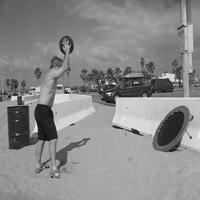
\includegraphics[width=2in]{frame_0074.jpg}
\caption{Still frame from video of man throwing ball.}
\label{fig:mana}
\end{minipage}\hfill
\begin{minipage}{0.33\textwidth}
\centering
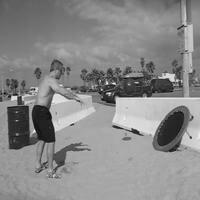
\includegraphics[width=2in]{frame_0076.jpg}
\caption{Still frame from video of man throwing ball.}
\label{fig:manb}
\end{minipage}
\begin{minipage}{0.33\textwidth}
\centering
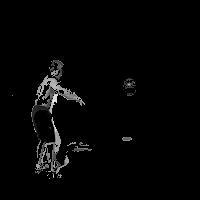
\includegraphics[width=2in]{median_man.jpg}
\caption{Still frame from video of median filter applied to video of man throwing ball.}
\end{minipage}
\end{figure*}


%
% The following two commands are all you need in the
% initial runs of your .tex file to
% produce the bibliography for the citations in your paper.
\bibliographystyle{abbrv}
\bibliography{bibliography}  % bibliography.bib is the name of the Bibliography in this case
% You must have a proper ".bib" file
%  and remember to run:
% latex bibtex latex latex
% to resolve all references
%
% ACM needs 'a single self-contained file'!
%
%\balancecolumns % GM June 2007
% That's all folks!
\end{document}
